\documentclass[11pt,a4paper]{article}
\usepackage[margin=24mm,headheight=15pt]{geometry}
\usepackage[T1]{fontenc}
\usepackage{lmodern,microtype,amsmath,amssymb,mathtools}
\usepackage{tikz,graphicx}
\usetikzlibrary{arrows.meta,positioning,calc,patterns}
\usepackage{booktabs,tabularx,array,enumitem}
\usepackage[font=small,labelfont=bf]{caption}
\captionsetup{hypcap=false}
\usepackage{xcolor,fancyhdr,titlesec}
\definecolor{ink}{HTML}{17324D}
\definecolor{teal}{HTML}{087F8C}
\definecolor{orange}{HTML}{BD622A}
\definecolor{muted}{HTML}{526575}
\usepackage[colorlinks=true,linkcolor=teal,urlcolor=teal,citecolor=teal]{hyperref}
\hypersetup{pdftitle={From Error Correction to Fault-Tolerant Computation},pdfauthor={}}
\newcommand{\ket}[1]{\lvert #1\rangle}
\newcommand{\SL}{\mathcal S}
\newcommand{\XL}{\overline X}
\newcommand{\ZL}{\overline Z}
\newcommand{\pL}{p_{\mathrm L}}
\newcommand{\cnot}{\operatorname{CNOT}}
\newcommand{\takeaway}[1]{\begin{quote}\color{ink}\textbf{#1}\end{quote}}
\setlength{\parindent}{0pt}
\setlength{\parskip}{5pt}
\setlength{\emergencystretch}{2em}
\titleformat{\section}{\Large\bfseries\color{ink}}{\thesection}{0.6em}{}
\titleformat{\subsection}{\large\bfseries\color{ink}}{\thesubsection}{0.6em}{}
\pagestyle{fancy}\fancyhf{}
\fancyhead[L]{\small\color{muted} QUANTUM COMPUTING / FOUNDATIONS}
\fancyfoot[L]{\small\color{muted} Tutorial 04: From Error Correction to Fault Tolerance}
\fancyfoot[R]{\small\thepage}
\renewcommand{\headrulewidth}{0.3pt}
\setlist[itemize]{itemsep=3pt,leftmargin=1.5em}
\setlist[enumerate]{itemsep=4pt,leftmargin=1.5em}
\tikzset{box/.style={draw=teal,rounded corners,align=center,minimum height=10mm,inner sep=5pt},arr/.style={-{Latex[length=2mm]},thick}}
\newcommand{\YL}{\overline Y}

\begin{document}
\begin{center}
{\small\color{teal}\textbf{QUANTUM ERROR CORRECTION / TUTORIAL 04}}\\[9pt]
{\LARGE\bfseries\color{ink} From Error Correction\\[3pt] to Fault-Tolerant Computation}\\[9pt]
{\large From a noisy CNOT to a reliable program}\\[6pt]
{\small Revised version / 30 September 2026}
\end{center}

The earlier tutorials used redundancy and parity checks to protect quantum information against Pauli errors. Notebook 1 introduced Shor's code and the correction of single-qubit Pauli errors. Notebook 2 made error correction geometrical through local surface-code checks and lattice surgery. It also added faults after ancilla--data gates, so check outcomes and raw logical readouts could already be wrong. Preparation, direct measurement readout, and idle periods remained ideal, and we recorded detector events without decoding them.

Those idealized steps are also places where a real computation can fail. Preparation may put a data qubit or ancilla in the wrong state, a qubit may suffer an error while waiting, and a direct measurement may report the wrong bit. Fault tolerance asks whether the entire logical computation still works when these faults occur alongside gate faults, provided their number is within the protection the implementation claims. To answer that, we must decode noisy measurement histories, limit how faults spread during logical operations, and use decoded results when later operations depend on them. This is the step from protecting stored information to protecting a program as it runs.

In this tutorial, we show how repeated checks form a syndrome volume and how detection events help us interpret faults during memory and lattice surgery. We then follow the consequences for a logical program: tracking corrections, using a decoded result to control a magic-state \(T\) gate, and identifying what a practical decoder must know and when it must respond. Finally, we define ways to assess logical failure and budget risk across the program. 

We follow one program throughout: prepare logical patches $C$ in $\ket+_L$ and $D$ in $\ket0_L$, protect them while they wait, perform a lattice-surgery CNOT, apply a logical $T$ to $C$, and measure both logical qubits in $X$. The $T$ gate will be defined when we reach it. We call the target patch $D$ to avoid confusing it with that gate.

\begin{center}
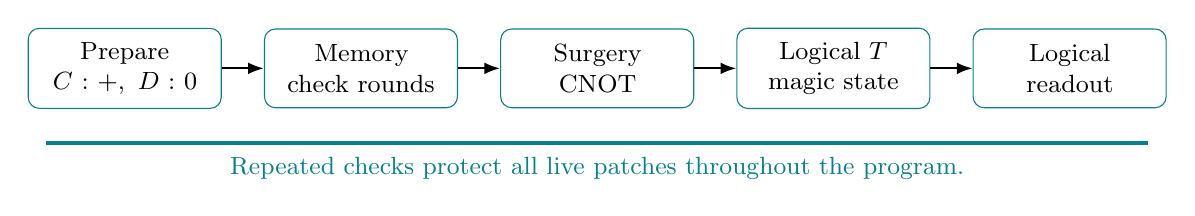
\begin{tikzpicture}[font=\small]
\foreach \x/\lab in {0/{Prepare\\$C:+,\ D:0$},3/{Memory\\check rounds},6/{Surgery CNOT},9/{Logical $T$\\magic state},12/{Logical\\readout}}{
\node[box,text width=2.1cm] (p\x) at (\x,0) {\lab};}
\foreach \a/\b in {0/3,3/6,6/9,9/12}{\draw[arr] (p\a)--(p\b);}
\draw[teal,very thick] (-1,-.95)--(13,-.95);
\node[teal,below] at (6,-1){Repeated checks protect all live patches throughout the program.};
\end{tikzpicture}
\captionof{figure}{The running program. Each logical stage expands into physical gates, repeated checks, and classical processing. The CNOT ancilla and magic-state supply need additional qubits.}
\label{fig:program}
\end{center}

% \section{The CNOT we know, with noisy measurements}\label{sec:noisy}
% Recall the four seam checks in Tutorial 03. Their product was the logical parity $\ZL_C\ZL_A$. If their ideal outcome bits are $g_1,\ldots,g_4$, the joint result is
% \[
% a=g_1\oplus g_2\oplus g_3\oplus g_4.
% \]
% One wrong reported $g_j$ flips this inferred parity. Increasing the patch size does not make that single readout trustworthy. We need evidence across time as well as across space. The first new ingredient is therefore a history of repeated, noisy checks~\cite{horsman}.

% \clearpage
\section{From noisy measurements to a spacetime history}\label{sec:volume}
As a logical patch waits, data and ancillas can suffer faults, and a check measurement can report the wrong sign. A memory experiment repeats the checks so that a single report need not decide the logical state.

Let $s_i(r)$ be the reported bit of check $i$ in round $r$, with $0$ denoting sign $+1$ and $1$ sign $-1$. For a check whose ideal sign should stay constant, compare adjacent reports:
\begin{equation}\label{eq:detector}
\delta_i(r)=s_i(r)\oplus s_i(r-1).
\end{equation}
 The value $\delta_i(r)=1$ is a \emph{detection event}: the expected relation between two reports has failed. It marks a change, not simply a check outcome of $1$. Placing these events at their check positions and measurement rounds gives a \emph{syndrome volume}~\cite{dennis,stim}.

\begin{center}
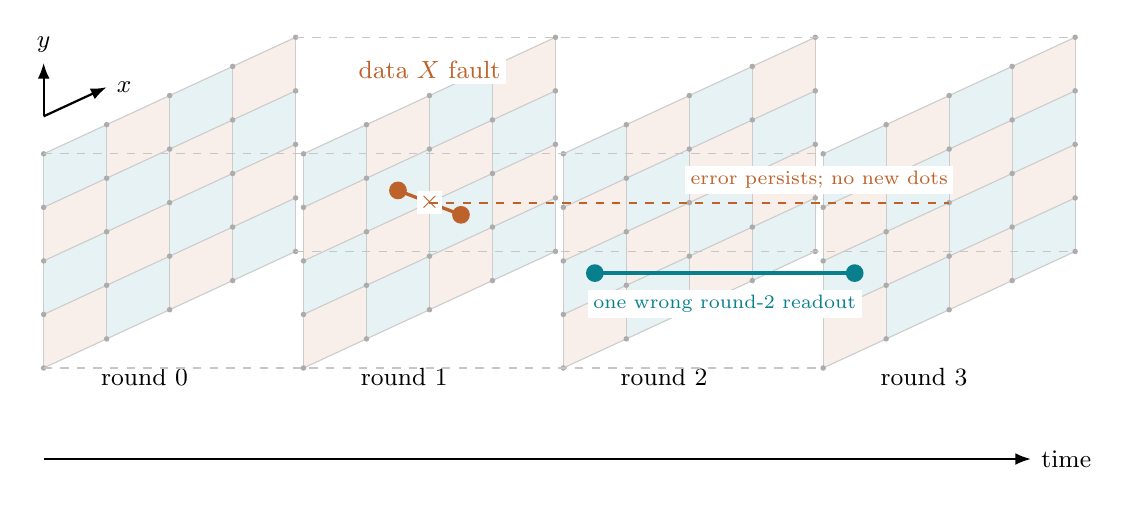
\begin{tikzpicture}[x={(.8cm,.37cm)},y={(0cm,.68cm)},z={(3.3cm,0cm)},font=\small]
% Physical x/y slices extend obliquely; z is the horizontal time coordinate.
\foreach \r in {0,1,2,3}{
 \foreach \i in {0,1,2,3}{\foreach \j in {0,1,2,3}{
  \pgfmathtruncatemacro{\parity}{mod(\i+\j,2)}
  \ifnum\parity=0 \fill[orange!10] (\i,\j,\r)--(\i+1,\j,\r)--(\i+1,\j+1,\r)--(\i,\j+1,\r)--cycle;
  \else \fill[teal!10] (\i,\j,\r)--(\i+1,\j,\r)--(\i+1,\j+1,\r)--(\i,\j+1,\r)--cycle;\fi
 }}
 \foreach \i in {0,...,4}{\draw[gray!40] (\i,0,\r)--(\i,4,\r);\draw[gray!40] (0,\i,\r)--(4,\i,\r);}
 \foreach \i in {0,...,4}{\foreach \j in {0,...,4}{\fill[gray!65] (\i,\j,\r) circle (1pt);}}
 \node[below] at (1.6,-.7,\r){round \r};
}
% Four corners connect the slices into a history volume.
\foreach \i/\j in {0/0,0/4,4/0,4/4}{\draw[gray!45,dashed] (\i,\j,0)--(\i,\j,3);}
% A central X fault affects the two teal Z plaquettes centered at (1.5,2.5),(2.5,1.5).
\draw[orange,very thick] (1.5,2.5,1)--(2.5,1.5,1);
\fill[orange] (1.5,2.5,1) circle (3.2pt);\fill[orange] (2.5,1.5,1) circle (3.2pt);
\node[orange,fill=white,inner sep=1pt] at (2,2,1){$\times$};
\node[orange,anchor=south,fill=white,inner sep=2pt] at (2,4.2,1){data $X$ fault};
\draw[orange,dashed,thick] (2,2,1)--(2,2,3);
\node[orange,anchor=south,fill=white,inner sep=2pt,font=\scriptsize] at (2,2.15,2.5){error persists; no new dots};
% A different Z check has one wrong outcome in round 2.
\draw[teal,very thick] (.5,1.5,2)--(.5,1.5,3);
\fill[teal] (.5,1.5,2) circle (3.2pt);\fill[teal] (.5,1.5,3) circle (3.2pt);
\node[teal,anchor=north,fill=white,inner sep=2pt,font=\scriptsize] at (.5,1.2,2.5){one wrong round-2 readout};
\draw[arr] (0,-1.7,0)--(0,-1.7,3.8) node[right]{time};
\draw[arr] (0,4.7,0)--(1,4.7,0) node[right]{$x$};
\draw[arr] (0,4.7,0)--(0,5.7,0) node[above]{$y$};
\end{tikzpicture}
\captionof{figure}{A surface-code memory history, with rounds 0--3 running left to right. Gray dots are data qubits; orange and teal faces are $X$ and $Z$ checks. Large dots mark changes in $Z$-check reports. In orange, a data $X$ fault gives two neighboring checks the history $0,1,1,1$. Their two round-1 events suggest a data error, which the decoder can track in its Pauli frame. In teal, one wrong readout gives a check the history $0,0,1,0$. Its round-2 and round-3 events suggest a bad report, with no data correction. Solid lines connect each event pair; the dashed line shows the persistent data error. Boundary checks and ancillas are omitted.}
\label{fig:volume}
\end{center}
The decoder uses a specified model of the check circuit to infer a plausible fault history from the detection events, then determines its possible logical effect. In the orange example, two neighboring $Z$ checks change between rounds 0 and 1, producing two events in the same round. Their signs then persist. A data $X$ fault explains the pair, so the decoder records an $X$ recovery in the Pauli frame. In the teal example, one check changes in round 2 and changes back in round 3, producing two events at the same location in consecutive rounds. One bad round-2 report explains this pattern, so the data frame remains unchanged.

This memory example was simple because each check kept the same support from one round to the next. A lattice-surgery CNOT changes that support as patches merge and split. We now extend the same history-based reasoning through those transitions.

% \clearpage
\subsection{From memory history to a protected CNOT}\label{sec:cnot}

Recall the three logical patches: control $C$, target $D$, and auxiliary patch $A$ prepared in $\ket+_L$. The CNOT uses the logical measurements
\[
\ZL_C\ZL_A
\ \longrightarrow\
\XL_A\XL_D
\ \longrightarrow\
\ZL_A.
\]
We call their decoded outcome bits $a$, $b$, and $c$. The first two are joint measurements, each made by merging and then splitting patches. The last is a logical $Z$ readout of $A$.

\begin{center}
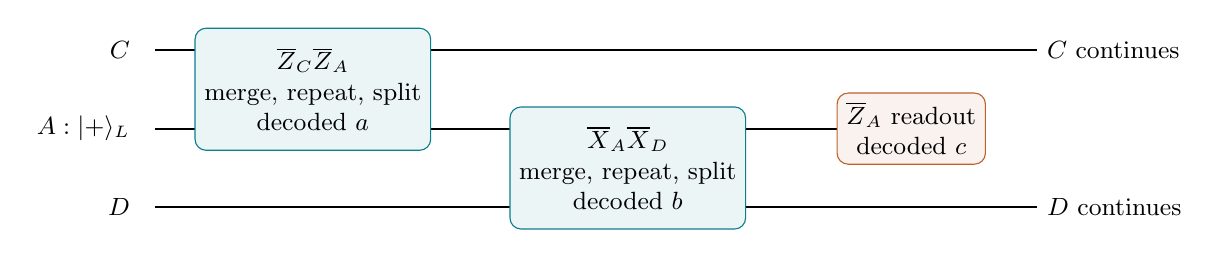
\begin{tikzpicture}[font=\small,x=1cm,y=1cm]
\node[anchor=east] at (0,2) {$C$};
\node[anchor=east] at (0,1) {$A:\ket+_L$};
\node[anchor=east] at (0,0) {$D$};
\draw[thick] (.2,2)--(11.4,2);
\draw[thick] (.2,1)--(9.7,1);
\draw[thick] (.2,0)--(11.4,0);
\node[draw=teal,rounded corners,fill=teal!8,align=center,
  minimum width=2.2cm,minimum height=1.55cm] at (2.2,1.5)
  {$\ZL_C\ZL_A$\\merge, repeat, split\\decoded $a$};
\node[draw=teal,rounded corners,fill=teal!8,align=center,
  minimum width=2.2cm,minimum height=1.55cm] at (6.2,.5)
  {$\XL_A\XL_D$\\merge, repeat, split\\decoded $b$};
\node[draw=orange,rounded corners,fill=orange!8,align=center,
  minimum width=1.6cm,minimum height=.72cm] at (9.8,1)
  {$\ZL_A$ readout\\decoded $c$};
\node[anchor=west] at (11.4,2) {$C$ continues};
\node[anchor=west] at (11.4,0) {$D$ continues};
\end{tikzpicture}
\captionof{figure}{Logical measurement sequence for the surgery CNOT. Each joint-measurement box stands for a merge with repeated seam checks followed by a split. The final readout measures patch $A$ and consumes it. All three bits are decoded using the check history and the running Pauli frame. The bridge qubits used during a merge are distinct from logical patch $A$.}
\label{fig:cnot-sequence}
\end{center}

Consider the first, $ZZ$, merge. In the bridge layout from Tutorial 03,
patches $C$ and $A$ are temporarily joined using bridge data qubits
$b_0,b_1,b_2$. Four new $Z$ seam checks $G_1,\ldots,G_4$ are measured,
and their product is $\ZL_C\ZL_A$. We do not know the individual seam-check
signs in advance. Their first results may be random even without a fault.
We therefore measure the checks for several rounds and use the history
to infer the joint outcome $a$. Once a seam check has been measured,
its sign should persist unless a fault changes it. If only occasional
readouts were wrong, inferring its sign would resemble choosing the
result reported most often. The full decoder also accounts for data
and gate faults.

After the merge interval, $C$ and $A$ must be separated so that $A$ can participate in the next joint measurement with $D$. We measure each bridge qubit once in $X$, obtaining bits $r_0,r_1,r_2$, and resume the original boundary checks. These bridge outcomes determine a split byproduct $D_{\mathbf r}$ in the Pauli frame, as derived in Tutorial 03. A bridge readout can be wrong, even though the qubit cannot simply be measured again after this destructive split.

The surrounding checks provide evidence about these single readouts. In the first merge, let $B_L$ and $B_R$ be the original $X$ boundary checks of $C$ and $A$. The corresponding merged checks are $H_L=B_LX_{b_0}X_{b_1}$ and $H_R=B_RX_{b_1}X_{b_2}$. Write $h_L,h_R$ for their last reported bits before the split, and $s_L,s_R$ for the first reports of $B_L,B_R$ after it. Every bit is $0$ for sign $+1$ and $1$ for sign $-1$. With no faults, the records obey
\[
\delta_L=h_L\oplus r_0\oplus r_1\oplus s_L=0,
\qquad
\delta_R=h_R\oplus r_1\oplus r_2\oplus s_R=0.
\]
If the only fault were one bridge readout flip, $r_0$ would trigger the left relation, $r_1$ both, and $r_2$ the right. In the full circuit, check reports and data can fail too. The decoder therefore uses repeated checks before and after the split and the circuit fault model to interpret this pattern. The two relations alone do not certify every bridge bit.

The second joint measurement follows the same plan in the complementary basis: merge $A$ with $D$, repeatedly measure the new $X$ seam checks to infer $b$ for $\XL_A\XL_D$, then split and decode that transition. Finally, measure the data qubits of $A$ once in $Z$. Their outcomes give a raw logical-$Z$ bit. The preceding compatible check history and current frame let the decoder interpret that readout as $c$.

After accounting for the split byproducts and inferred recoveries, the decoded bits $a,b,c$ determine the CNOT's logical byproduct
\begin{equation}\label{eq:cnotframe}
F=\ZL_C^{\,b}\XL_D^{\,a\oplus c}.
\end{equation}
Here $F$ is the byproduct of the measurement-based CNOT. The running Pauli frame also contains the split byproducts $D_{\mathbf r}$ and any inferred recoveries. Those entries must be propagated consistently when interpreting $a,b,c$ and later readouts.

To some extent, repeated checks protect the measurement outcomes, but repetition alone
does not make the CNOT fault tolerant. We also use the N- and Z-shaped
check-extraction schedules introduced in Tutorial 03 to limit hook-error
propagation in the merged patches. The decoder must retain the valid
relations across both merges and splits, as well as noisy preparation
and final readout. These circuit and decoding choices must be checked
together before claiming a particular level of fault protection.

% \clearpage
\section{Clifford gates and the universal gate set}\label{sec:frame}
The Pauli frame is a classical record of corrections we have inferred but have not physically applied. To carry this record through a gate, we need to know what happens to a pending Pauli correction when the gate acts. Some gates turn it into another Pauli correction, so we can simply update the record. These are called Clifford gates. The \(T\) gate does not always do this, which means a Pauli frame alone may no longer be enough. We will see how this distinction affects correction and readout, why Clifford gates together with \(T\) form a universal gate set, and how to implement a logical \(T\) using a magic state.

A \textbf{Clifford gate} $U$ is a gate for which $UPU^\dagger$ is another Pauli for every Pauli $P$, including products of Paulis on several qubits. Hadamard $H$, the phase gate $S=\operatorname{diag}(1,i)$, and CNOT are typical examples. Applying $U$ gives
\begin{equation}\label{eq:frame}
UP\ket\psi=(UPU^\dagger)U\ket\psi.
\end{equation}
Thus the intended gate acts while the controller replaces its record $P$ with $UPU^\dagger$. Suppose the intended state is $\ket{\psi}$, but a known $Z$ error
means the stored state is $Z\ket{\psi}$. We want the result of applying $H$ to the intended state, namely $H\ket{\psi}$. If we apply $H$
directly to the stored state, we obtain
\[
HZ\ket{\psi}=XH\ket{\psi},
\]
because $HZH=X$. The output therefore has a known $X$ error. We
update the Pauli frame from $Z$ to $X$ and continue, rather than
physically correcting the $Z$ before the Hadamard or applying an $X$
afterward. If we subsequently measure logical $Z$, the tracked $X$ reverses
the reported bit because $X$ anticommutes with $Z$. An $X$
measurement needs no reversal.

However, Clifford gates alone do not give universal quantum computation. A standard extension is the $T$ gate,
\[
T=\operatorname{diag}(1,e^{i\pi/4}),\qquad
T(\alpha\ket0+\beta\ket1)=\alpha\ket0+e^{i\pi/4}\beta\ket1.
\]
It adds a $45^\circ$ relative phase to the $\ket1$ component, and $T^2=S$. The Clifford set supplies CNOT, an entangling gate, while $H$ and $T$ together approximate arbitrary single-qubit gates. This is why Clifford gates together with $T$ can approximate arbitrary quantum circuits~\cite{gottesman,fowler}. But $T$ is not Clifford:
\[
TXT^\dagger=(X+Y)/\sqrt2,
\]
so a Pauli-only record is no longer sufficient. Our next step shows one way to perform a logical $T$, and exactly where its decoded measurement result affects the hardware.

% \clearpage
\section{Apply a logical \texorpdfstring{$T$}{T} using a magic state}
\label{sec:magic}

We want to apply $\overline T$ to logical patch $C$. We do not apply
a physical $T$ gate to every data qubit. Instead, we consume a second
logical patch $M$ prepared in the magic state
\[
\ket M_L=\overline T\ket+_L
=\frac{\ket{0_L}+e^{i\pi/4}\ket{1_L}}{\sqrt2}.
\]
The phase $e^{i\pi/4}$ in this resource is what the procedure transfers
to $C$. Supplying a sufficiently accurate $\ket M_L$ is a separate
task~\cite{magic,fowler}.

There are three steps. First, perform the lattice-surgery logical CNOT
from $C$ (control) to $M$ (target). Second, measure $M$ in logical $Z$.
Third, use its decoded, frame-adjusted outcome $k$ to decide whether
$C$ needs an $\overline S$ correction. Patch $C$ remains the output.
Patch $M$ is measured and consumed.

We do not repeat the whole injection to vote on $k$. Its logical
outcome is random, and measuring $M$ consumes the patch. Instead,
check measurements continue through the CNOT and up to the readout
of $M$. The data qubits of $M$ are then measured in $Z$ once. The
decoder combines those physical outcomes with the preceding check
history and known frame to infer $k$. An incorrect inference selects
the wrong $\overline S$ branch.

\begin{center}
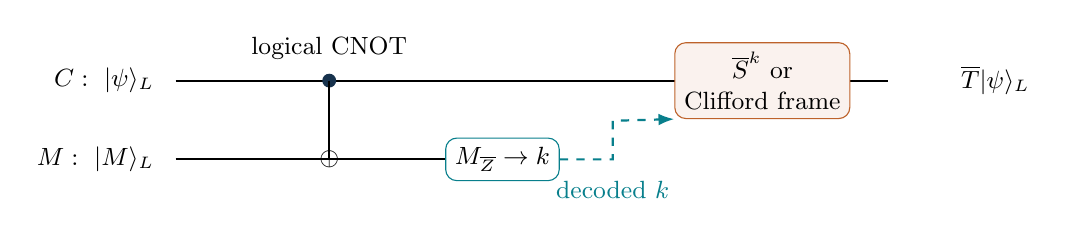
\begin{tikzpicture}[font=\small]
\node[anchor=east] at (0,1) {$C:\ \ket\psi_L$};
\node[anchor=east] at (0,0) {$M:\ \ket M_L$};
\draw[thick] (.15,1)--(9.2,1);
\draw[thick] (.15,0)--(4.7,0);

\fill[ink] (2.1,1) circle (2.5pt);
\draw[thick] (2.1,1)--(2.1,0);
\node at (2.1,0) {$\oplus$};
\node[above] at (2.1,1.15) {logical CNOT};

\node[draw=teal,rounded corners,fill=white] (meas)
  at (4.3,0) {$M_{\ZL}\to k$};
\node[draw=orange,rounded corners,fill=orange!8,align=center,
  minimum width=2.05cm,minimum height=.8cm] (corr)
  at (7.6,1) {$\overline S^k$ or\\Clifford frame};
\draw[teal,dashed,-{Latex[length=2mm]},thick]
  (meas.east) -- (5.7,0) -- (5.7,.49) -- (corr.south west);
\node[teal,below] at (5.7,-.15) {decoded $k$};
\node[anchor=west] at (10,1) {$\overline T\ket\psi_L$};
\end{tikzpicture}
\captionof{figure}{Magic-state injection of a logical $T$. The decoded logical-$Z$ result $k$ of $M$ controls a physical $\overline S$ when $k=1$, or an equivalent Clifford-frame update. The CNOT symbol denotes the protected surgery protocol of Figure~\ref{fig:cnot-sequence}; using that protocol also needs an auxiliary patch $A$, omitted from these two logical wires. Patch $M$ is consumed.}
\label{fig:t-injection}
\end{center}

\textbf{Why does this implement $\overline T$ on $C$?}
Let $\omega=e^{i\pi/4}$ and write the magic state on patch $M$ as
\[
\ket M_L
=\frac{\ket{0_L}+\omega\ket{1_L}}{\sqrt2}.
\]
The subscript $L$ marks an encoded state. A subscript $M$ on an
operator or bra identifies the patch on which it acts.
On patch $C$, define the projectors onto the two logical basis states:
\[
P_0=\frac{I+\ZL_C}{2},
\qquad
P_1=\frac{I-\ZL_C}{2}.
\]
The ideal logical CNOT acts as
\[
U=P_0\otimes I_M+P_1\otimes\XL_M.
\]
Thus $M$ is flipped when $C$ is in $\ket{1_L}$ and is unchanged when
$C$ is in $\ket{0_L}$.

After the CNOT, measure $M$ in logical $Z$. Taking the overlap with
$\ket{0_L}_M$ or $\ket{1_L}_M$ leaves an operator on $C$. To calculate
these operators, note that
\[
\XL_M\ket M_L
=\frac{\ket{1_L}+\omega\ket{0_L}}{\sqrt2}.
\]
The two measurement branches are therefore
\begin{align}
K_0
&={}_M\langle 0_L|U|M\rangle_L
 =\frac{P_0+\omega P_1}{\sqrt2}
 =\frac{\overline T_C}{\sqrt2},
\notag\\
K_1
&={}_M\langle 1_L|U|M\rangle_L
 =\frac{\omega P_0+P_1}{\sqrt2}
 =\frac{\omega\overline T_C^\dagger}{\sqrt2}.
\label{eq:branches}
\end{align}
Here $\overline T_C=P_0+\omega P_1$. The factors of $1/\sqrt2$
give each ideal outcome probability $1/2$, while the overall factor
$\omega$ in the second branch has no observable effect.

Outcome $k=0$ already applies $\overline T_C$. For $k=1$, apply
$\overline S_C$, since
\[
\overline S_C K_1
=\frac{\omega\overline S_C\overline T_C^\dagger}{\sqrt2}
=\frac{\omega\overline T_C}{\sqrt2}.
\]
With the correct decoded value of $k$, both branches therefore
implement $\overline T_C$ on patch $C$.

\subsection{Correct now, or adapt the next operation}

In the $k=1$ branch, patch $C$ holds, up to a global phase,
\[
\overline T^\dagger\ket\psi
=\overline S^\dagger\overline T\ket\psi.
\]
The intended state is $\overline T\ket\psi$, so there is a known
extra $\overline S^\dagger$. We can remove it by applying
$\overline S$ now. We can also defer that gate and record
$\overline S^\dagger$ in a \emph{Clifford frame}~\cite{slowframe}.

Deferring the gate is valid only if we account for this frame when
performing later operations. Before an affected operation, the
controller must either apply $\overline S$ or adapt that operation.
It cannot always wait until the end and change a recorded bit.

Our running program makes the choice concrete. The next intended
operation on $C$ is a logical-$X$ measurement. If $k=1$, we can:
\begin{enumerate}
\item Apply $\overline S$, then measure $\XL_C$; or
\item Leave $\overline S$ deferred, then measure
\[
\overline S^\dagger\XL_C\overline S=-\YL_C.
\]
This means measuring logical $Y$ and reversing its reported sign.
\end{enumerate}
If $k=0$, there is no $\overline S$ correction, so we measure
$\XL_C$ as planned.

Why must we decide before measuring? An intended $\ket+_L$ gives
a certain $X$ result, but $\overline S^\dagger\ket+_L$ gives random
$X$ results. Flipping those recorded bits afterward cannot recover
the intended result. If the device cannot perform a protected
logical-$Y$ measurement, we must apply $\overline S$ before its
logical-$X$ measurement.

The conditional logical $S$ and optional logical-$Y$ readout are assumed to be protected operations. Their physical schedules and failure probabilities belong in an assessment of the complete program.

The decoded bit $k$ must therefore be ready before the conditional
$\overline S$ or the affected measurement-basis choice. While the
controller waits, patch $C$ continues its check cycles. If no
upcoming physical operation depends on $k$, decoding may finish
later.

\subsection{Follow the running program}

Figure~\ref{fig:program-loop} follows the same patches through our
program. Each row shows a quantum procedure, the measurements it
produces, and what the classical decoder or controller does with them.
Time runs downward. A frame update is a change to a classical record,
not automatically a correction gate.

\begin{center}
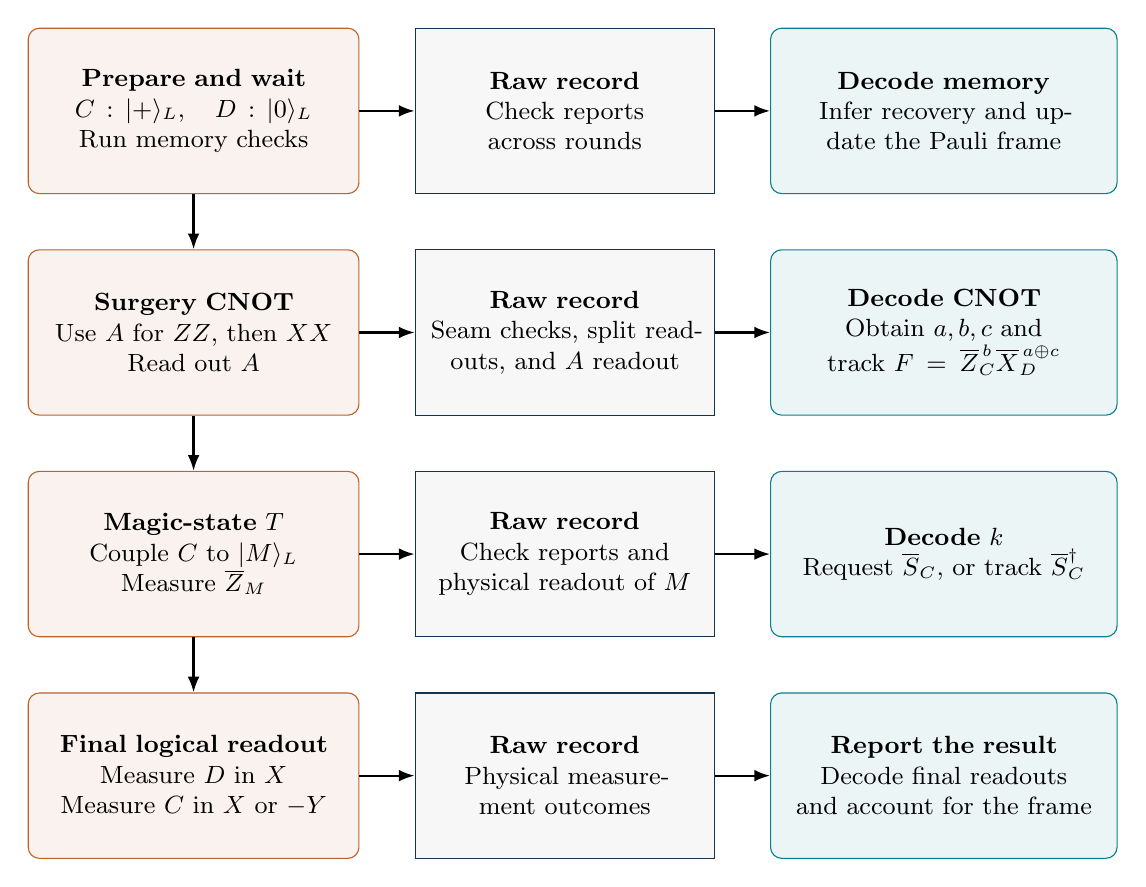
\begin{tikzpicture}[
  font=\small,
  quantum/.style={
    draw=orange,fill=orange!8,rounded corners,
    align=center,text width=3.8cm,minimum width=4.2cm,
    minimum height=21mm,inner sep=0pt
  },
  record/.style={
    draw=ink,fill=gray!6,
    align=center,text width=3.4cm,minimum width=3.8cm,
    minimum height=21mm,inner sep=0pt
  },
  classical/.style={
    draw=teal,fill=teal!8,rounded corners,
    align=center,text width=4.0cm,minimum width=4.4cm,
    minimum height=21mm,inner sep=0pt
  }
]
\node[quantum] (q0)
  {\textbf{Prepare and wait}\\
   $C:\ket+_L,\quad D:\ket0_L$\\
   Run memory checks};
\node[record,right=7mm of q0] (r0)
  {\textbf{Raw record}\\
   Check reports across rounds};
\node[classical,right=7mm of r0] (c0)
  {\textbf{Decode memory}\\
   Infer recovery and update the Pauli frame};

\node[quantum,below=7mm of q0] (q1)
  {\textbf{Surgery CNOT}\\
   Use $A$ for $ZZ$, then $XX$\\
   Read out $A$};
\node[record,right=7mm of q1] (r1)
  {\textbf{Raw record}\\
   Seam checks, split readouts,
   and $A$ readout};
\node[classical,right=7mm of r1] (c1)
  {\textbf{Decode CNOT}\\
   Obtain $a,b,c$ and track
   $F=\ZL_C^{\,b}\XL_D^{\,a\oplus c}$};

\node[quantum,below=7mm of q1] (q2)
  {\textbf{Magic-state $T$}\\
   Couple $C$ to $\ket M_L$\\
   Measure $\ZL_M$};
\node[record,right=7mm of q2] (r2)
  {\textbf{Raw record}\\
   Check reports and
   physical readout of $M$};
\node[classical,right=7mm of r2] (c2)
  {\textbf{Decode $k$}\\
   Request $\overline S_C$, or track
   $\overline S_C^\dagger$};

\node[quantum,below=7mm of q2] (q3)
  {\textbf{Final logical readout}\\
   Measure $D$ in $X$\\
   Measure $C$ in $X$ or $-Y$};
\node[record,right=7mm of q3] (r3)
  {\textbf{Raw record}\\
   Physical measurement
   outcomes};
\node[classical,right=7mm of r3] (c3)
  {\textbf{Report the result}\\
   Decode final readouts and
   account for the frame};

% Measurements flow to classical processing within each stage.
\draw[arr] (q0)--(r0); \draw[arr] (r0)--(c0);
\draw[arr] (q1)--(r1); \draw[arr] (r1)--(c1);
\draw[arr] (q2)--(r2); \draw[arr] (r2)--(c2);
\draw[arr] (q3)--(r3); \draw[arr] (r3)--(c3);

% The quantum program progresses downward and then ends.
\draw[arr] (q0.south)--(q1.north);
\draw[arr] (q1.south)--(q2.north);
\draw[arr] (q2.south)--(q3.north);
\end{tikzpicture}
\captionof{figure}{The running program, from protected preparation
to final logical readout. Orange boxes are quantum procedures, gray
boxes are their raw measurement records, and teal boxes show classical
decoding and control. Each row's decoded information accompanies the
patches into the next stage. In the simplified $k=1$ branch shown here,
the controller either applies $\overline S_C$ or defers it and later
measures $-\YL_C$ instead of $\XL_C$. Other tracked byproducts must
also be included when interpreting the final results.}
\label{fig:program-loop}
\end{center}

During memory, the decoder uses changes in repeated check reports to
infer likely faults. It records recovery information in the Pauli
frame while the physical patches continue their check cycles.

The surgery CNOT produces noisy seam, split, and auxiliary-patch readout records. Decoding them gives the logical bits $a,b,c$ and the known CNOT byproduct $F$. The frame also carries split byproducts and inferred recoveries. That full record must accompany $C$ and $D$ into the next stage. The
magic-state procedure then produces another decoded bit, $k$.
If $k=1$, the controller can apply $\overline S_C$ or retain
$\overline S_C^\dagger$ in a Clifford frame. In the latter case it
must choose the corresponding physical basis before $C$ is measured.

Finally, the physical readout bits are decoded and interpreted using
the accumulated frame to obtain the intended logical-$X$ outcomes.
The controller need not apply every tracked correction as a gate.
It does need the relevant decoded information before any physical
gate or measurement basis that depends on it.

\section{What a practical decoder must do}\label{sec:decoders}
Figure~\ref{fig:program-loop} gives the decoder a concrete job. It must track errors while $C$ and $D$ wait, interpret the surgery outcomes $a,b,c$, infer the magic-state outcome $k$, and correct the final logical readouts. The controller then combines those results with the current frame. It does not automatically apply the decoder's inferred recovery as physical gates.

\subsection{Build a model of the full measurement record}
The decoder receives raw check reports and any scheduled data measurements. To turn them into detection events, it must know which parity relations should hold without faults. That requires the actual check schedule, preparation and readout boundaries, and the changes at each merge and split. Equation~\eqref{eq:detector} works for a check that persists unchanged. Across a surgery transition, valid relations can involve several reports, as in the split detector of Section~\ref{sec:cnot}~\cite{stim}.

The readout of $M$ is especially important. Its logical $Z$ outcome $k$ is random, so a result of $1$ is not itself an error. We do not repeat the whole $T$ procedure to vote on it. Instead, the data qubits of $M$ are measured once in $Z$. Those physical bits give a raw logical parity and close the histories of compatible checks measured before readout. The decoder uses any resulting detection events, together with the known frame, to infer whether that raw parity must be flipped. It performs analogous interpretation for the readout of $A$ and for the final measurements of $C$ and $D$. The final model must include whichever $X$ or $Y$ protocol the controller actually selected for $C$.

Preparation also supplies a boundary for the history. For example, initializing every data qubit in $\ket+$ fixes the initial $X$-check signs to $+1$, but leaves the $Z$-check signs undetermined. A noisy first $X$-check report can be tested against that expected sign and later reports. The decoder must use only such valid initial relations for the actual preparation circuit.

A useful circuit model also lists possible fault mechanisms and what each would do to detectors and logical observables. Preparation, idle, gate, and readout faults need not have equal rates. One faulty two-qubit gate can produce correlated data errors and several detector events. A physical $Y$ has linked $X$ and $Z$ components. Treating these effects as unrelated can lose information. Leakage needs additional information or physical handling because a Pauli-frame update cannot return a leaked qubit to the computational subspace~\cite{leakage}.

\subsection{Infer the logical effect, not just an event pattern}
The same detection events can have more than one fault explanation. In a simple memory with data error $E$ and inferred Pauli recovery $R$, the inference succeeds on an arbitrary logical state when $RE$ is a stabilizer, up to phase. If $RE$ is a nontrivial logical operator, every detection event may be accounted for while the logical information is still wrong. For our program, a wrong inference of $k$ can likewise select the wrong $\overline S$ branch or the wrong final basis.

\begin{center}
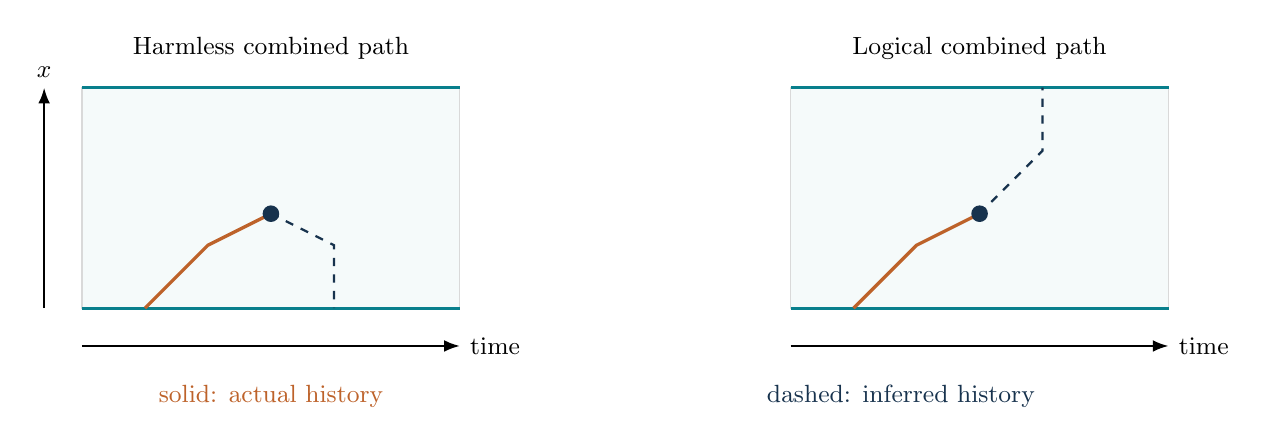
\begin{tikzpicture}[x=.8cm,y=.8cm,font=\small]
\foreach \shift/\title in {0/{Harmless combined path},9/{Logical combined path}}{
 \begin{scope}[xshift=\shift cm]
 \fill[teal!4] (0,0) rectangle (6,3.5);
 \draw[gray!30] (0,0) rectangle (6,3.5);
 \draw[teal,very thick] (0,0)--(6,0) (0,3.5)--(6,3.5);
 \draw[orange,very thick] (1,0)--(2,1)--(3,1.5);
 \fill[ink] (3,1.5) circle (3pt);
 \node[above,align=center] at (3,3.8){\title};
 \draw[arr] (0,-.6)--(6,-.6) node[right]{time};
 \end{scope}
}
\draw[ink,dashed,thick] (3,1.5)--(4,1)--(4,0);
\begin{scope}[xshift=9cm]
\draw[ink,dashed,thick] (3,1.5)--(4,2.5)--(4,3.5);
\end{scope}
\draw[arr] (-.6,0)--(-.6,3.5) node[above]{$x$};
\node[orange] at (3,-1.4){solid: actual history};
\node[ink] at (13,-1.4){dashed: inferred history};
\end{tikzpicture}
\captionof{figure}{A spatial--time slice for one check type in a planar memory; the other spatial coordinate is suppressed. Both candidate histories explain the black event. On the left, actual plus inferred paths return to the same absorbing boundary. On the right, they connect opposite absorbing boundaries and act logically. The horizontal teal lines are spatial boundaries extended through time.}
\label{fig:paths}
\end{center}

The figure illustrates why a decoder must choose a \emph{logical effect}, not merely connect every event to something. A minimum-weight decoder selects one compatible fault configuration that minimizes a model-dependent cost. For an independent binary mechanism with probability $q_e$, a common edge weight is $w_e=\log[(1-q_e)/q_e]$. Maximum-likelihood logical-class decoding instead adds the probabilities of all configurations with the same logical effect. The most likely single configuration need not belong to the most likely class.

Sparse Blossom, available through PyMatching, is one practical minimum-weight matching decoder~\cite{matching}. Its graph represents a fault mechanism by an edge joining two detectors, or one detector and an allowed boundary. Edges also record any logical-observable flips. This is useful for graph-like error models, but pairwise matching cannot exactly represent every correlated mechanism that produces more than two events. Decomposition or a richer method must handle such mechanisms explicitly. Belief-matching is one way to use correlated fault information before matching~\cite{belief}. Whichever decoder is chosen, test its logical accuracy on the actual surgery and readout circuits, not only on a static memory.

\subsection{Keep enough history and meet the decision deadline}
A long program may be decoded in overlapping windows. Suppose one bad check report creates detection events in rounds 4 and 5. A window ending at round 4 sees only half the evidence. It must keep the newer rounds as context or pass the unresolved event to the next window.

\begin{center}
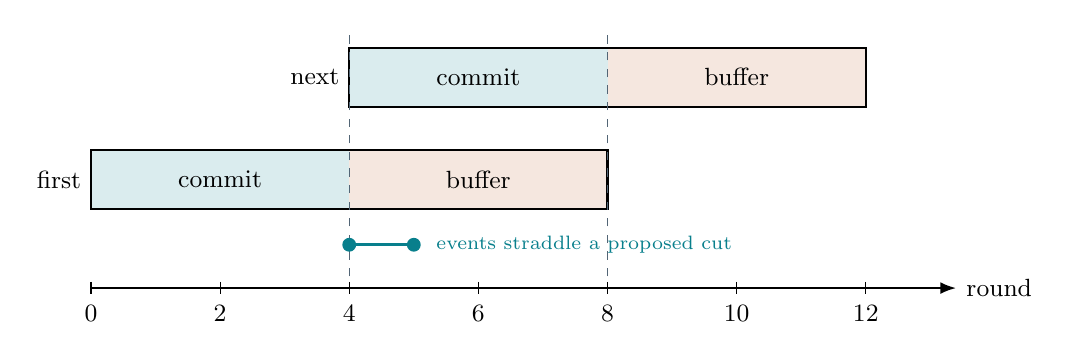
\begin{tikzpicture}[x=.82cm,y=1cm,font=\small]
\draw[arr] (0,0)--(13.4,0) node[right]{round};
\foreach \r in {0,2,4,6,8,10,12}{
  \draw (\r,.08)--(\r,-.08);
  \node[below] at (\r,-.1){\r};
}
\fill[teal!15] (0,1) rectangle (4,1.75);
\fill[orange!15] (4,1) rectangle (8,1.75);
\draw[thick] (0,1) rectangle (8,1.75);
\node at (2,1.38){commit};
\node at (6,1.38){buffer};
\fill[teal!15] (4,2.3) rectangle (8,3.05);
\fill[orange!15] (8,2.3) rectangle (12,3.05);
\draw[thick] (4,2.3) rectangle (12,3.05);
\node at (6,2.68){commit};
\node at (10,2.68){buffer};
\node[left] at (0,1.38){first};
\node[left] at (4,2.68){next};
\draw[muted,dashed] (4,.15)--(4,3.3) (8,.15)--(8,3.3);
\draw[teal,very thick] (4,.55)--(5,.55);
\fill[teal] (4,.55) circle (2.5pt);
\fill[teal] (5,.55) circle (2.5pt);
\node[anchor=west,teal,font=\scriptsize] at (5.2,.55)
  {events straddle a proposed cut};
\end{tikzpicture}
\captionof{figure}{An illustrative sliding window. Decode eight rounds, commit the older four, and retain the newer four as context. Events near a window edge may be explained by later evidence. These sizes illustrate the method and are not a general distance prescription.}
\label{fig:windows}
\end{center}

The decoder must carry unresolved events and the boundary information induced by committed decisions into the next window. A software cutoff is not a physical boundary where a fault chain can simply end. Windows that cross a merge or split must also retain the detector relations connecting both sides~\cite{windows}.

Two timing measures now matter. \emph{Throughput} is how much record the decoder processes per unit time. It must keep up with the continuing check stream. \emph{Latency} is the delay until a particular decoded result is available, including data acquisition, buffering, processing, and communication. A decoder could keep up on average yet return $k$ too late for the conditional $\overline S$ or the later $X$ versus $-Y$ basis choice.

For illustration, a worker receiving one block every $1\,\mu\mathrm{s}$ but taking $1.2\,\mu\mathrm{s}$ per block develops a growing queue. Even a faster worker can miss a decision deadline if its window buffer adds too much delay. Waiting is possible only while live patches continue protected check cycles, and the extra exposure belongs in the program's failure budget. Decoder accuracy, throughput, and latency are separate requirements. We next define which logical failures they must help prevent and how to budget their risk.

\section{Define and budget the program's failure}\label{sec:budget}
The preceding section described what the decoder must infer and when it must return an answer. We now need to say what counts as a failure before assigning that decoder or the program an error rate. A wrong $a,b,c$, a wrong $k$, and a wrong final readout can have different effects, so one memory curve cannot stand for the entire computation.

\subsection{First choose a test with a definite meaning}
For the running program, ideal preparation and CNOT create a Bell pair. Applying $T$ to $C$ gives
\[
\ket{\Psi_T}=\frac{\ket{00}_L+e^{i\pi/4}\ket{11}_L}{\sqrt2},
\qquad \langle\XL_C\XL_D\rangle=\frac1{\sqrt2}.
\]
The individual $X$ results are random. Even their product is $-1$ with probability $(1-1/\sqrt2)/2$ in the ideal program. Such a shot is not a logical failure. Comparing many shots with the predicted correlation tests one feature of the output distribution, but does not assign a right-or-wrong label to each shot or characterize the whole logical channel. Later, $P_{\rm fail}$ means the probability of a harmful logical event in a specified fault model, not the frequency of an ideally random measurement outcome.

For a binary diagnostic with a definite ideal answer, stop a separate test after the CNOT and measure both patches in $Z$. Prepare $\ket+_C\ket0_D$, specify a fixed noisy preparation, storage interval, physical surgery schedule, final readout, and decoder. The ideal decoded parity is $z_C\oplus z_D=0$. Define
\begin{equation}\label{eq:pL}
p_L^{ZZ}(p)=\Pr[\text{decoded final }ZZ\text{ parity is odd}].
\end{equation}
This is a probability \emph{per complete test}, including preparation, the CNOT, and readout. A separate $XX$ test probes a complementary error sector. These tests are useful diagnostics, not a characterization of an arbitrary-input CNOT or of the later $T$ procedure. A full claim needs suitable input/output tests or circuit-level verification of the logical map and its adaptive branches.

Under a stochastic Pauli model, simulations can label faults by logical effect and estimate these diagnostic rates. Stim supports the stabilizer preparation, checks, surgery, and readout parts~\cite{stim}. The non-stabilizer magic state and its contribution to the full program need an additional simulation method or a justified resource-state error model. A memory error curve alone cannot supply the full-program rate.

\subsection{Why the lowest-order failing faults set the slope}
Once the test and its decoder are fixed, the small-noise slope has a precise meaning. Fix a finite circuit with $N$ fault locations and a fixed decoder, including tie breaking. For this derivation, each location fails independently with probability $p$. The conditional distribution of its fault type is fixed: for example, a failed CNOT applies a uniformly random nonidentity two-qubit Pauli, and a failed readout flips its report. Let $\Lambda$ be the exact set of faulty locations and $q_{\Lambda}$ the conditional chance that the chosen test fails, averaged over fault types and measurement randomness. Then
\begin{equation}\label{eq:exact}
p_L(p)=\sum_{\Lambda\subseteq\{1,\ldots,N\}}q_{\Lambda}\,p^{|\Lambda|}(1-p)^{N-|\Lambda|}.
\end{equation}
If every set smaller than $m$ succeeds and at least one $m$-fault set can fail, the first nonzero terms give
\begin{align}
p_L(p)&=p^m(1-p)^{N-m}\sum_{|\Lambda|=m}q_{\Lambda}+O(p^{m+1})\notag\\
&=\alpha_m p^m+O(p^{m+1}),\qquad \alpha_m=\sum_{|\Lambda|=m}q_{\Lambda}.\label{eq:scaling}
\end{align}
The last step uses fixed $N$ and $(1-p)^{N-m}=1+O(p)$ as $p\to0$. $\alpha_m$ counts weighted harmful configurations; it is not automatically $\binom Nm$.

% \clearpage
\subsection{A countable example from our seam}
The four seam checks of the distance-three $ZZ$ merge from Tutorial 03 give a small example whose leading coefficient we can count. This is a deliberately restricted readout experiment, not the failure rate of the surgery CNOT. Assume the four true check signs stay fixed, all preparation and quantum operations are ideal, and only reported check bits flip independently with probability $p$. Report each of the four checks three times and take a majority vote for each sign. One majority is wrong with probability
\[
q=\binom32p^2(1-p)+p^3=3p^2-2p^3.
\]
The inferred joint parity is wrong if an odd number of those four majorities is wrong. Its exact failure probability is
\begin{align}
p_{\rm seam}&=4q(1-q)^3+4q^3(1-q)\notag\\
&=\frac{1-(1-2q)^4}{2}=12p^2+O(p^3).\label{eq:seamrate}
\end{align}
There are 12 two-readout failure pairs that first cause failure: three possible pairs in each of four checks. Here $m=2$ and $\alpha_2=12$. With only one report per check, the parity failure would instead be $[1-(1-2p)^4]/2=4p+O(p^2)$.

This restricted calculation shows exactly what three reports buy under independent readout flips. In the actual CNOT, data faults can change check signs persistently, gate faults create correlations, and checks appear or disappear at merges and splits. A new seam check can also have a random initial sign. Independent majority votes are therefore not a decoder for the full operation. Its $q_{\Lambda}$, $m$, and $\alpha_m$ must be established from the specified circuit and decoder.

If an operation and decoder really tolerate every allowed set of up to $t$ circuit faults, their chosen failure test has no terms below order $t+1$. Conversely, a surviving single-fault failure produces a linear contribution. Passing one observable test can hide another logical error sector, so test the claimed logical action and composability conditions as well as its measured slope.

For unequal rates $p_\ell=c_\ell p$, with fixed $c_\ell$, the same argument weights each leading fault set by $\prod_{\ell\in\Lambda}c_\ell$. Correlations between locations, leakage, coherent errors, or a decoder whose rule changes with $p$ need their own analysis. The expansion applies as $p\to0$ for a fixed circuit; it does not establish a scalable threshold on its own.

For circuits too large to enumerate, sample full noisy shots and report $n_{\rm fail}/n$ failures with statistical uncertainty. With no failures in $n$ independent shots, an approximate 95\% upper bound is $3/n$, not zero risk. Below we use illustrative curves to explain how to read rates, not as measured performance of our circuit.

% \clearpage
\subsection{Read a crossing only after defining the comparison}
A low-noise slope tells us how many faults first defeat a \emph{fixed} test. A crossing makes a different comparison and is meaningful only when both implementations perform the same task. Equation~\eqref{eq:scaling} gives $\log p_L\simeq\log\alpha_m+m\log p$: the low-noise log--log slope is $m$. Compare encoded and unencoded implementations of the \emph{same} CNOT parity test, with the same input, output criterion, and wall-clock duration. The unencoded implementation includes the corresponding idle time. In Figure~\ref{fig:thresholds}(a), choose the illustrative normalization $p_{\rm bare}=p$ and a hypothetical encoded curve $p_{\rm enc}=100p^2$.

\begin{center}
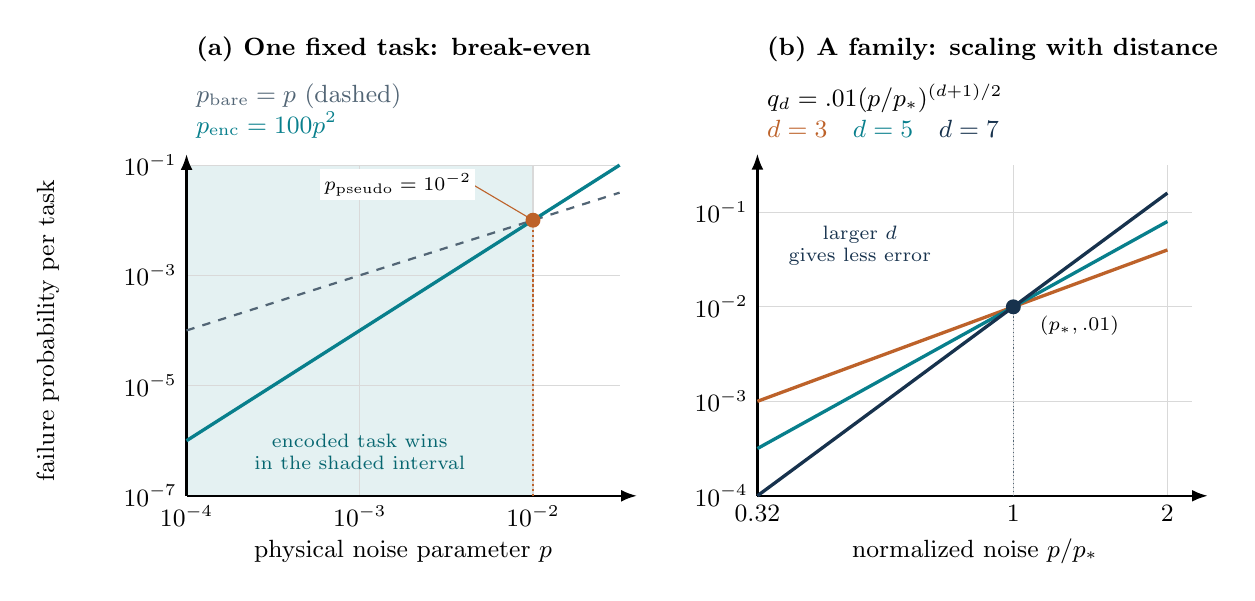
\begin{tikzpicture}[font=\small]
\begin{scope}[x=2.2cm,y=.7cm]
\node[font=\small\bfseries,anchor=west] at (0,8.1){(a) One fixed task: break-even};
\node[anchor=north west,align=left] at (0,7.65){\textcolor{muted}{$p_{\rm bare}=p$ (dashed)}\\\textcolor{teal}{$p_{\rm enc}=100p^2$}};
\fill[teal!11] (0,0)--(2,0)--(2,6)--(0,6)--cycle;
\foreach \x/\lab in {0/{10^{-4}},1/{10^{-3}},2/{10^{-2}}}{\draw[gray!30] (\x,0)--(\x,6);\node[below] at (\x,0){$\lab$};}
\foreach \y/\lab in {0/{10^{-7}},2/{10^{-5}},4/{10^{-3}},6/{10^{-1}}}{\draw[gray!30] (0,\y)--(2.5,\y);\node[left] at (0,\y){$\lab$};}
\draw[arr] (0,0)--(2.6,0);\draw[arr] (0,0)--(0,6.2);
\draw[muted,dashed,thick] (0,3)--(2.5,5.5);
\draw[teal,very thick] (0,1)--(2.5,6);
\draw[orange,densely dotted,thick] (2,0)--(2,5);
\fill[orange] (2,5) circle (2.7pt);
\draw[orange,thin] (2,5)--(1.65,5.65);
\node[anchor=east,fill=white,inner sep=1.5pt,font=\scriptsize] at (1.67,5.65){$p_{\rm pseudo}=10^{-2}$};
\node[teal!80!black,font=\scriptsize,align=center] at (1,.8){encoded task wins\\in the shaded interval};
\node at (1.25,-1){physical noise parameter $p$};
\node[rotate=90] at (-.8,3){failure probability per task};
\end{scope}
\begin{scope}[shift={(10.5cm,0)},x=6.5cm,y=1.2cm]
\node[font=\small\bfseries,anchor=west] at (-.5,4.725){(b) A family: scaling with distance};
\node[anchor=north west,align=left] at (-.5,4.4625){$q_d=.01(p/p_*)^{(d+1)/2}$\\\textcolor{orange}{$d=3$}\quad\textcolor{teal}{$d=5$}\quad\textcolor{ink}{$d=7$}};
\foreach \x/\lab in {-.5/{0.32},0/{1},.30103/{2}}{\draw[gray!30] (\x,0)--(\x,3.5);\node[below] at (\x,0){$\lab$};}
\foreach \y/\lab in {0/{10^{-4}},1/{10^{-3}},2/{10^{-2}},3/{10^{-1}}}{\draw[gray!30] (-.5,\y)--(.35,\y);\node[left] at (-.5,\y){$\lab$};}
\draw[arr] (-.5,0)--(.38,0);\draw[arr] (-.5,0)--(-.5,3.62);
\draw[orange,very thick] (-.5,1)--(.30103,2.60206);
\draw[teal,very thick] (-.5,.5)--(.30103,2.90309);
\draw[ink,very thick] (-.5,0)--(.30103,3.20412);
\draw[muted,densely dotted] (0,0)--(0,2);
\fill[ink] (0,2) circle (2.7pt);
\node[anchor=west,font=\scriptsize,fill=white,inner sep=2pt] at (.04,1.8){$(p_*,.01)$};
\node[align=center,font=\scriptsize,ink] at (-.3,2.65){larger $d$\\gives less error};
\node at (-.075,-.5833){normalized noise $p/p_*$};
\end{scope}
\end{tikzpicture}
\captionof{figure}{Two distinct comparisons, using illustrative curves rather than data. (a) The bare and encoded implementations perform the same CNOT parity test for the same duration, with the illustrative normalization $p_{\rm bare}=p$. The dot marks their only positive crossing. (b) Three illustrative probabilities per completed CNOT parity test in a family of distance-$d$ implementations cross at $(p_*,0.01)$. Their ordering reverses across that point. These power-law guides apply only to the plotted range; $p_*$ is illustrative, not a measured hardware threshold.}
\label{fig:thresholds}
\end{center}

Their positive crossing at $p=10^{-2}$ is a \textbf{pseudothreshold}: this particular encoded test wins against its specified bare comparator to the left. A comparison with one bare gate would be meaningless if the encoded rate included a much longer program. Nor should a low-$p$ approximation be extrapolated to a crossing unless it remains accurate there.

A \textbf{scalable threshold} asks whether increasing protection can make logical failures arbitrarily rare under the given noise model, circuit family, and decoding scheme. Figure~\ref{fig:thresholds}(b) instead compares distances for one completed logical test; each curve includes that implementation's duration. Better ordering at larger distance is the relevant trend. Finite-distance crossings may drift and require scaling analysis~\cite{dennis}. Memory protection alone also leaves the program's other operations to be established.

% \clearpage
\subsection{Give the complete program a risk budget}
The CNOT parity diagnostic leaves out memory, magic-state delivery, the decoded branch bit $k$, and final readout. To reason about the whole running program, let $E_j$ be a harmful logical event assigned to stage $j$. Choose events so that, if none happens, the intended logical computation and output distribution are preserved. If $\Pr(E_j)\leq p_j$ in the composed program, then
\begin{equation}\label{eq:union}
P_{\rm fail}\leq \Pr\!\left(\bigcup_j E_j\right)\leq\sum_j p_j.
\end{equation}
This is a bound, not an equality, and it does not require independence. The stage bounds must include allowed incoming errors, adaptive branches, and the agreed noise assumptions. A clean-input benchmark alone may not supply that guarantee~\cite{agp}.

For an illustrative target $P_{\rm fail}\leq10^{-3}$, suppose validation supplies the following conservative bounds. These numbers are hypothetical allocations, not performance claims for a device or decoder.
\begin{center}
\begin{tabularx}{\linewidth}{@{}Xlr@{}}
\toprule
Stage & Assumed bound & Contribution\\
\midrule
Prepare $C,D$ & $2\times10^{-5}$ each & $4\times10^{-5}$\\
Wait: 2 patches, 10 rounds & $10^{-6}$ per patch-round & $2\times10^{-5}$\\
Surgery CNOT, including $A$ & $6\times10^{-5}$ per operation & $6\times10^{-5}$\\
Deliver the magic state & $3\times10^{-5}$ per state & $3\times10^{-5}$\\
Consume it and implement the branch & $4\times10^{-5}$ per operation & $4\times10^{-5}$\\
Protected final readout of $C,D$ & $10^{-5}$ each & $2\times10^{-5}$\\
\midrule
Total & & $P_{\rm fail}\leq2.1\times10^{-4}$\\
\bottomrule
\end{tabularx}
\captionof{table}{One way to allocate risk across the running program. Each bound applies to its complete stated stage. Under these assumptions, the sum meets the illustrative target.}
\label{tab:budget}
\end{center}

The memory term multiplies a bound on a harmful event \emph{per patch-round} by 20 patch-rounds. The gate terms already cover their internal check rounds and the memory of other live patches during those stages. Do not count that exposure twice. The magic-state consumption bound includes an incorrectly decoded $k$ or an incorrect conditional $\overline S$ or basis choice. The final-readout bound covers the $X$ or $Y$ protocol actually selected. Likewise, the complete-test probability in Eq.~\eqref{eq:pL} already includes its preparation and readout. It cannot be inserted as a pure CNOT rate and then have those errors added again.

Waiting for a decoder or a factory must be assigned somewhere too. For example, an extra 20 rounds on each of two live patches adds at most $40\times10^{-6}$ under the same uniform per-round assumption. If the deferred-$S$ implementation changes the final basis to $Y$, its readout bound must cover that protected protocol, not just an easier $X$ readout.

The program now has an operational acceptance test. Its physical operations must satisfy the claimed fault-propagation and composition conditions, its decoder must interpret the chosen circuit and noise model accurately enough, its controller must meet the actual deadlines, and the validated stage bounds must meet the program target. For scalable fault tolerance, increasing resources must continue reducing logical risk across the required operations. This tutorial identifies those requirements and illustrates how to test them. It does not certify a particular surgery circuit or decoder. The extra checks, ancillas, resource states, classical processing, and verification are what turn an ideal logical construction into a fault-tolerant program.

\clearpage
\begin{thebibliography}{99}
\setlength{\itemsep}{4pt}
\bibitem{horsman} D. Horsman, A. G. Fowler, S. Devitt, and R. Van Meter, \emph{Surface code quantum computing by lattice surgery}, New J. Phys. \textbf{14}, 123011 (2012).\newline
\href{https://arxiv.org/abs/1111.4022}{arXiv:1111.4022}.
\bibitem{terhal} B. M. Terhal, \emph{Quantum error correction for quantum memories}, Rev. Mod. Phys. \textbf{87}, 307--346 (2015).\newline
\href{https://arxiv.org/abs/1302.3428}{arXiv:1302.3428}.
\bibitem{magic} S. Bravyi and A. Kitaev, \emph{Universal quantum computation with ideal Clifford gates and noisy ancillas}, Phys. Rev. A \textbf{71}, 022316 (2005).\newline
\href{https://arxiv.org/abs/quant-ph/0403025}{arXiv:quant-ph/0403025}.
\bibitem{fowler} A. G. Fowler, M. Mariantoni, J. M. Martinis, and A. N. Cleland, \emph{Surface codes: Towards practical large-scale quantum computation}, Phys. Rev. A \textbf{86}, 032324 (2012).\newline
\href{https://arxiv.org/abs/1208.0928}{arXiv:1208.0928}.
\bibitem{leakage} M. McEwen et al., \emph{Removing leakage-induced correlated errors in superconducting quantum error correction}, Nature Communications \textbf{12}, 1761 (2021).\newline
\href{https://arxiv.org/abs/2102.06131}{arXiv:2102.06131}.
\bibitem{agp} P. Aliferis, D. Gottesman, and J. Preskill, \emph{Quantum accuracy threshold for concatenated distance-3 codes}, Quantum Inf. Comput. \textbf{6}, 97--165 (2006).\newline
\href{https://arxiv.org/abs/quant-ph/0504218}{arXiv:quant-ph/0504218}.
\bibitem{gottesman} D. Gottesman, \emph{An Introduction to Quantum Error Correction and Fault-Tolerant Quantum Computation} (2009).\newline
\href{https://arxiv.org/abs/0904.2557}{arXiv:0904.2557}.
\bibitem{stim} C. Gidney, \emph{Stim: a fast stabilizer circuit simulator}, Quantum \textbf{5}, 497 (2021).\newline
\href{https://arxiv.org/abs/2103.02202}{arXiv:2103.02202}.
\bibitem{dennis} E. Dennis, A. Kitaev, A. Landahl, and J. Preskill, \emph{Topological quantum memory}, J. Math. Phys. \textbf{43}, 4452--4505 (2002).\newline
\href{https://arxiv.org/abs/quant-ph/0110143}{arXiv:quant-ph/0110143}.
\bibitem{windows} L. Skoric et al., \emph{Parallel window decoding enables scalable fault tolerant quantum computation}, Nature Communications \textbf{14}, 7040 (2023).\newline
\href{https://www.nature.com/articles/s41467-023-42482-1}{doi:10.1038/s41467-023-42482-1}.
\bibitem{matching} O. Higgott and C. Gidney, \emph{Sparse Blossom: correcting a million errors per core second with minimum-weight matching}, Quantum \textbf{9}, 1600 (2025).\newline
\href{https://quantum-journal.org/papers/q-2025-01-20-1600/}{doi:10.22331/q-2025-01-20-1600}.
\bibitem{belief} O. Higgott, T. C. Bohdanowicz, A. Kubica, S. T. Flammia, and E. T. Campbell, \emph{Improved Decoding of Circuit Noise and Fragile Boundaries of Tailored Surface Codes}, Phys. Rev. X \textbf{13}, 031007 (2023).\newline
\href{https://arxiv.org/abs/2203.04948}{arXiv:2203.04948}.
\bibitem{slowframe} C. Chamberland, P. Iyer, and D. Poulin, \emph{Fault-tolerant quantum computing in the Pauli or Clifford frame with slow error diagnostics}, Quantum \textbf{2}, 43 (2018).\newline
\href{https://quantum-journal.org/papers/q-2018-01-04-43/}{doi:10.22331/q-2018-01-04-43}.
\end{thebibliography}
\end{document}
